\documentclass[12pt,a4paper,oneside]{book} 
\usepackage[utf8]{inputenc}
\usepackage[spanish]{babel}
\usepackage{amsmath}
\usepackage{amsfonts}
\usepackage{amssymb}
\usepackage{graphicx}
\usepackage[left=2.54cm,right=2.54cm,top=2.54cm,bottom=2.54cm]{geometry}

\begin{document}
	
	\thispagestyle{empty} 
	
	\begin{center} 
		\LARGE{UNIVERSIDAD PRIVADA DE TACNA} \\[0.5cm] \Large{FACULTAD DE INGENIERÍA DE SISTEMAS}\\[0.5cm] \large{ ESCUELA PROFESIONAL DE INGENIERÍA SISTEMAS} 
	\end{center}
	
	\begin{figure}[htb]
		\centering 
\includegraphics[width=5cm, height=7cm]{img/uptlogo.png}
	\end{figure}
	
	\begin{center} \LARGE{\bf Informe N 03:}\\ \vspace{.25cm} { 
			\Large \bfseries {Instalación y Gestión de una base de datos MongoDB }}\\ 
		
	\end{center}
	
	\large{\bf Curso: } Base de Datos II
	\textbf{(SI-775)}\\
	\large{\bf Docente: } Ing. Patrick Cuadros Quiroga\\
	\large{\bf Alumno: } Liendo Velásquez , Joaquin\\
	\large{\bf Codigo: } 2016054463\\
	
	
	
	\begin{center} 
		\Large \textsc{Tacna - Perú} \\
		\Large \textsc{2020 } 
	\end{center}



	\newpage
	\begin{itemize}
		\item {Obtener el instalador para Windows (https://www.mongodb.com/download-center/community).}\\
		
		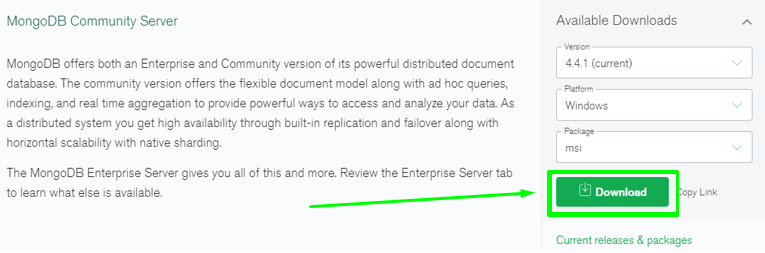
\includegraphics[width=16cm, height=5cm]{img/1.png}\\

	\item {Iniciar el instalador como administrador.}\\
	
	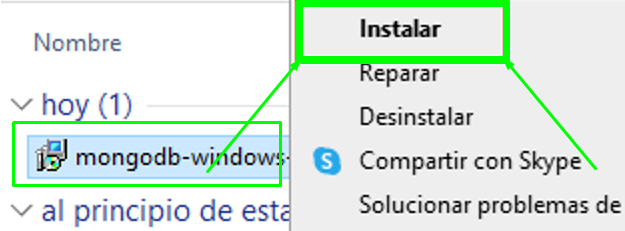
\includegraphics[width=16cm, height=4cm]{img/2.png}\\
	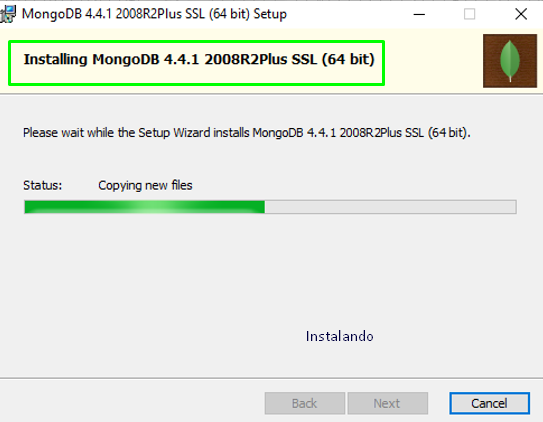
\includegraphics[width=16cm, height=10cm]{img/3.png}\\
	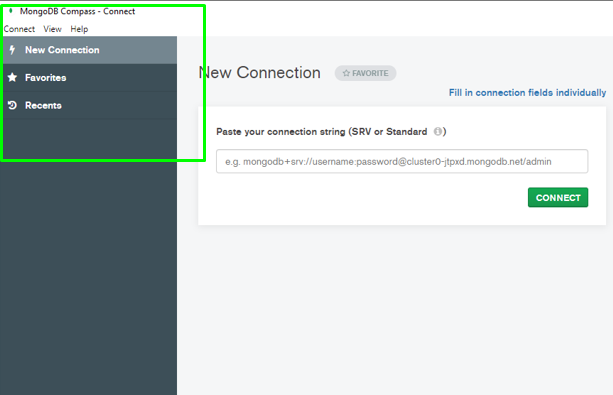
\includegraphics[width=16cm, height=10cm]{img/4.png}\\
	
		\item {Crear las carpetas de almacenamiento y configuracion de MongoDB.\\
		Dar permisos escritura y lectura a estas carpetas.\\
		C:/data \\
		C:/data/db \\
		}\\
	
	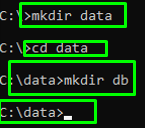
\includegraphics[width=8cm, height=5cm]{img/5.png}\\
	
\end{itemize}


	\newpage
\begin{itemize}
	\item {(Opcional) Crear las carpetas de almacenamiento en una ruta segura ejemplo: \\
	D:/mongodb/data/db}\\
	
	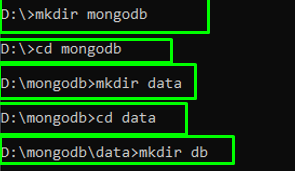
\includegraphics[width=16cm, height=9cm]{img/6.png}\\
	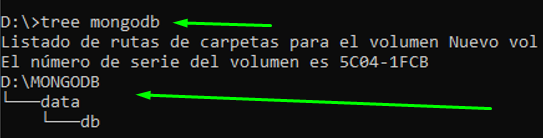
\includegraphics[width=16cm, height=9cm]{img/7.png}\\
	
	
\end{itemize}


	\newpage
\begin{itemize}
	\item {Iniciar el servidor del servicio de MongoDB: mongod. \\ C:/mongodb/bin/mongod.exe}\\
	
	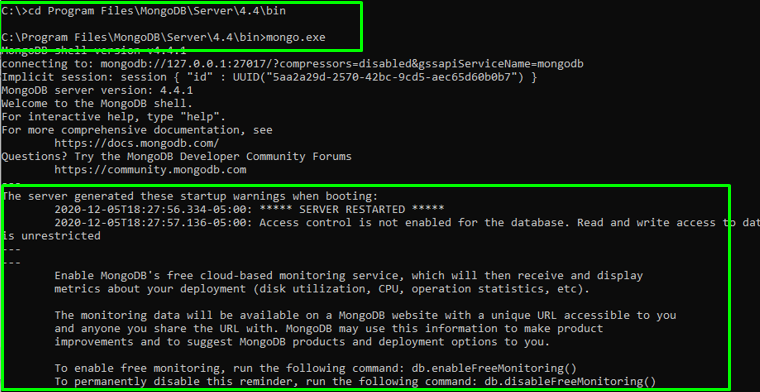
\includegraphics[width=16cm, height=9cm]{img/8.png}\\
	
	\item {Iniciar el Shell de mongo.\\ 
	C:/mongodb/bin/mongo.exe}\\
	
	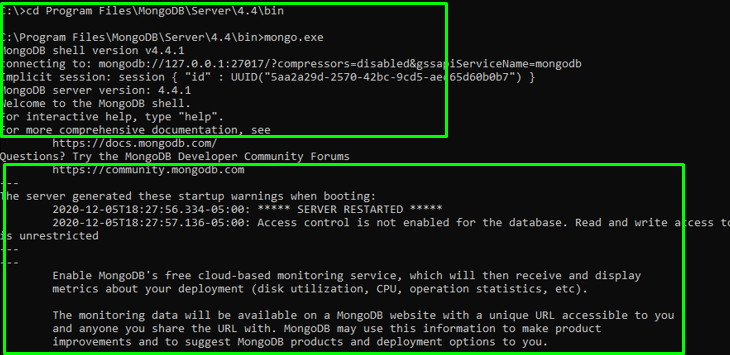
\includegraphics[width=16cm, height=9cm]{img/9.png}\\
	
	
\end{itemize}


	\newpage
\begin{itemize}
	\item {Iniciar el Shell de mongo.\\
		C:/mongodb/bin/mongo.exe
	}\\
	
	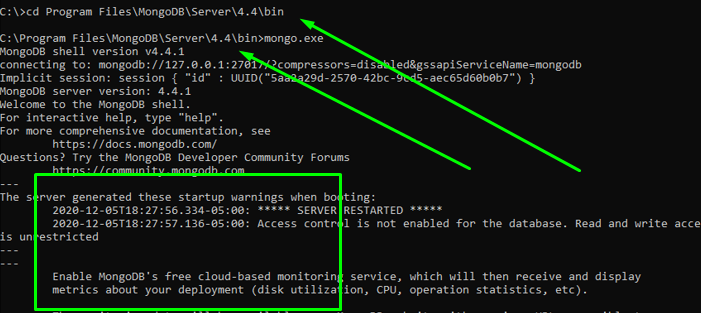
\includegraphics[width=16cm, height=9cm]{img/10.png}\\
	
	\item {Para realizar consultas a la base de datos, deberemos usar el comando d b.nombre\_de\_coleccion.find(). Este comando puede recibir dos parámetros: una consulta y una proyección. Ambos comandos son opcionales por lo que si ejecutamos el comando:\\
		
	db.people.find()
	 }\\
	
	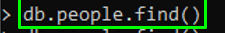
\includegraphics[width=16cm, height=4cm]{img/11.png}\\
	
	
\end{itemize}

	\newpage
\begin{itemize}
	\item {Obtendremos una larga lista con los primeros 20 elementos de la colección. Digo primeros, porque MongoDB no muestra todos los elementos. Para la consulta MongoDB crea un cursor. De todas formas al ejecutar el comando podemos ver que el resultado no está demasiado formateado, por lo que es muy difícil leerlo. Para solucionar este problema podemos usar el modificador pretty que nos devolverá un resultado mucho más legible.\\
		
	db.people.find().pretty()
	}\\
	
	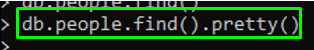
\includegraphics[width=16cm, height=4cm]{img/12.png}\\
	
	
	
	\item {11.	Ahora vamos a añadir la consulta al comando find, para que filtre los elementos según nuestras necesidades. Para ello especificaremos un objeto JSON como primer parámetro del comando, con los campo por los que queremos filtrar:\\
		
		db.people.find(\\
		{age:34}\\
		).pretty()
	
	
	}\\	
	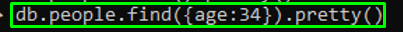
\includegraphics[width=16cm, height=4cm]{img/13.png}\\
	
	
\end{itemize}


	\newpage
\begin{itemize}
	\item {Con ese comando obtendremos las personas cuya edad es de 34 años. Podemos añadir tantos filtros como queramos.\\
		 db.people.find(\\
		{age:34,isActive:true}\\
		).pretty()
		
		
	}\\	
	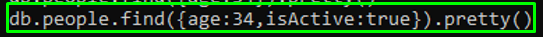
\includegraphics[width=16cm, height=2cm]{img/14.png}\\
	
	
	
	\item {En este caso filtramos por age y por isActive. Como se ve los resultados nos muestran todos los campos de cada elemento. Es como si hubiésemos utilizado el asterisco en una consulta SELECT. Si queremos seleccionar solo algunos de los campos, deberemos utilizar el segundo parámetro de la consulta find para definir una proyección. \\
		db.people.find(\\
		{age:34,isActive:true},\\
		{name:1,age:1,isActive:1}\\
		).pretty()	
		
	}\\	
	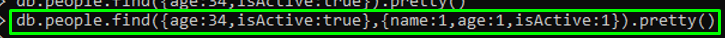
\includegraphics[width=16cm, height=2cm]{img/15.png}\\
	
	
	\item {Que nos devuelve solo los campos que se requieren, además del \_id. El \_id por defecto se muestra siempre, así que si queremos ocultarlo hay que especificarlo en la proyección.\\
		
		db.people.find(\\
		{age:34,isActive:true},\\
		{name:1,age:1,isActive:1,\_id:0}\\
		).pretty()
			
		
	}\\	
	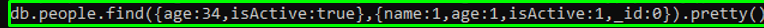
\includegraphics[width=16cm, height=2cm]{img/16.png}\\
	
	
\end{itemize}


	\newpage
\begin{itemize}
	\item {Si queremos mostrar todos los campos, pero quitando solo algunos, lo que haremos será desactivar los no deseados en la proyección:\\
		
		db.people.find(\\
		{age:34,isActive:true},\\
		{name:0,age:0,isActive:0,\_id:0}\\
		).pretty()
		
	}\\
	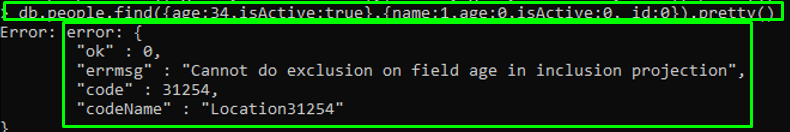
\includegraphics[width=16cm, height=5cm]{img/17.png}\\
	
	
	
	\item {16.	El comando findOne tiene el mismo funcionamiento que el comando find, con la diferencia de que, si el comando encuentra más de un resultado que cumpla las condiciones de la consulta, tan solo nos devolverá el primero.\\
		
		db.people.findOne(\\
		{age:34,isActive:true},\\
		{name:0,age:0,isActive:0,\_id:0}
		)
		
		
	}\\	
	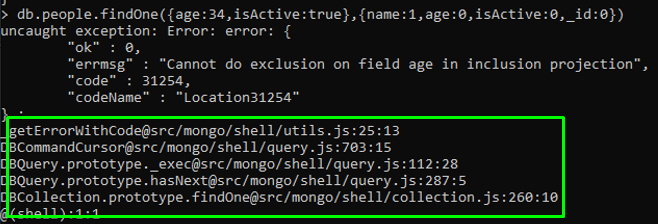
\includegraphics[width=16cm, height=8cm]{img/18.png}\\

	\item {Además findOne no acepta pretty, pero ya devuelve el resultado formateado.}\\
	
	\item {Se  percataran  de  que MongoDB  guarda  los  elementos  con  comillas  dobles  en   el   identificador.  Es   decir que MongoDB guarda las duplas “name”:“Helen” o “age”:34. En las consultas, en cambio, no se ha especificado dichas comillas. Esto es porque el motor JavaScript de MongoDB se encarga de añadirlas. Esto nos facilita la escritura de consultas, ya que no son obligatorias. De hecho, la siguiente consulta, funcionará perfectamente:\\
		
		db.people.findOne(\\
		{“age”:34,”isActive”:true},\\
		{“name”:0,”age”:0,”isActive”:0,”\_id”:0}\\
		)
	}\\
	
	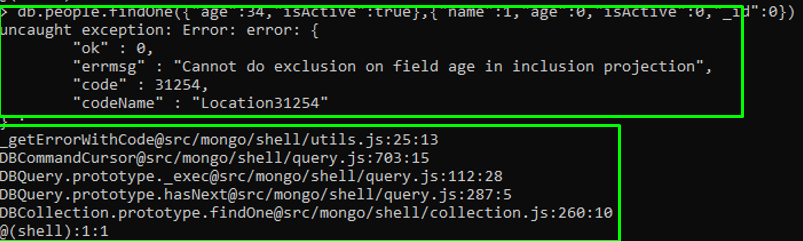
\includegraphics[width=16cm, height=4cm]{img/19.png}\\
	
\end{itemize}
	

	
\end{document}